\documentclass{article}
\title{MAT1105 Oblig 1}
\author{borgebj}
\date{}

\usepackage[norsk]{babel}
\usepackage{subcaption}
\usepackage{amsmath}
\usepackage{graphicx}
\usepackage[a4paper, top=1in, bottom=1in, left=1in, right=1in]{geometry}
\usepackage{subcaption}
\usepackage{float}

\maketitle

\setlength{\parskip}{2em}
\setlength{\parindent}{0pt}
\linespread{1}


\begin{document}

\section*{Seksjon 1.5}

\subsection*{Oppgave 5}

a) 
\[A = \begin{pmatrix}
    1 & 0 & -3 \\
    -2 & -3 & 2
\end{pmatrix} 
\quad \text{og} \quad \textbf{x} = \begin{pmatrix}
    -2\\3\\1
\end{pmatrix}\]

\[A\textbf{b} = \begin{pmatrix}
    1 \cdot (-2) + 0 \cdot 3 + (-3) \cdot 1\\
    (-2) \cdot (-2) + -3 \cdot 3 + 2 \cdot 1
\end{pmatrix} = \begin{pmatrix}
    -2 + 0 + 3 \\ 4 - 9 - 2
\end{pmatrix} = \underline{\begin{pmatrix}
    1\\7
\end{pmatrix}}\]



b) 
\[A = \begin{pmatrix}
    2 & 0  \\
    3 & 1 \\
    6 & -2
\end{pmatrix} 
\quad \text{og} \quad \textbf{x} = \begin{pmatrix}
    3\\-2
\end{pmatrix}\]

\[A\textbf{x} = \begin{pmatrix}
    2 \cdot 3 + 0 \cdot (-2) \\ 3 \cdot 3 + 1 \cdot (-2) \\ 6 \cdot 3 + (-2) \cdot ( -2)
\end{pmatrix} = \begin{pmatrix}
    6 + 0 \\ 9 - 2 \\ 18 + 4
\end{pmatrix} = \underline{\begin{pmatrix}
    6 \\ 7 \\ 22
\end{pmatrix}}\]


c)
\[A = \begin{pmatrix}
    2 & 1 & 0 \\ -3 & 4 & -2 \\ 1 & -3 & 2
\end{pmatrix} \quad \textbf{x} = \begin{pmatrix}
    4 \\ 0 \\ 3
\end{pmatrix}\]

\[A\textbf{x} = \begin{pmatrix}
    (2 \cdot 4) + (1 \cdot 0) + (0 \cdot 3) \\ ((-3) \cdot 4) + (4 \cdot 0) + ((-2) \cdot 3) \\ (1 \cdot 4) + (-3) \cdot 0 + (2 \cdot 3)
\end{pmatrix} = \begin{pmatrix}
    8 + 0 + 0 \\ -12 + 0 - 6 \\ 4 + 0 + 6
\end{pmatrix} = \underline{\begin{pmatrix}
    8 \\ -18 \\ 10
\end{pmatrix}}\]

\newpage

\subsection*{Oppgave 7}

\[A = \begin{pmatrix}
    0.7 & 0.3 & 0.4 \\ 0.1 & 0.5 & 0.2 \\ 0.2 & 0.2 & 0.4
\end{pmatrix} \quad \textbf{b} = \begin{pmatrix}
    50 \\ 70 \\ 80
\end{pmatrix}\]

\[
    A\textbf{b} = \begin{pmatrix}
        0.7 \cdot 50 + 0.3 \cdot 70 + 0.4 \cdot 80 \\ 0.1 \cdot 50 + 0.5 \cdot 70 + 0.2 \cdot 80 \\ 0.2 \cdot 50 + 0.2 \cdot 70 + 0.4 \cdot 80
    \end{pmatrix}
    =
    \begin{pmatrix}
        35 + 21 + 32 \\ 5 + 35 + 16 \\ 10 + 14 + 32
    \end{pmatrix}
    =
    \begin{pmatrix}
        88 \\ 56 \\ 56
    \end{pmatrix}
\]



\[\underline{X = 88 \qquad Y = 56 \qquad Z = 56}\]


\hfill
\hfill

\section*{Seksjon 1.6}

\subsection*{Oppgave 6}

\[A = \begin{pmatrix}
    0 & 1 \\ 0 & 2
\end{pmatrix}, \quad 
B = \begin{pmatrix}
    1 & 1 \\ 3 & 4
\end{pmatrix}, \quad
C = \begin{pmatrix}
    2 & 5 \\ 3 & 4
\end{pmatrix}, \quad
D = \begin{pmatrix}
    3 & 7 \\ 0 & 0
\end{pmatrix}\]

\[AB = \begin{pmatrix}
    0 \cdot 1 + 1 \cdot 3 & 0 \cdot 1 + 1 \cdot 4 \\ 0 \cdot 1 + 2 \cdot 3 & 0 \cdot 1 + 2 \cdot 4
\end{pmatrix} = \underline{\begin{pmatrix}
    3 & 4 \\ 6 & 8
\end{pmatrix}}\]

\[AC = \begin{pmatrix}
    0 \cdot 2 + 1 \cdot 3 & 0 \cdot 5 + 1 \cdot 4 \\ 0 \cdot 2 + 2 \cdot 3 & 0 \cdot 5 + 2 \cdot 4
\end{pmatrix} = \underline{\begin{pmatrix}
    3 & 4 \\ 6 & 8
\end{pmatrix}}\]

\[AD = \begin{pmatrix}
    0 \cdot 3 + 1 \cdot 0 & 0 \cdot 7 + 1 \cdot 0 \\ 0 \cdot 3 + 2 \cdot 0 & 0 \cdot 7 + 2 \cdot 0
\end{pmatrix} = \underline{\begin{pmatrix}
    0 & 0 \\ 0 & 0
\end{pmatrix} = 0}\]

\newpage

\subsection*{Oppgave 14}

\begin{figure}[H]
\centering
\begin{subfigure}{.5\textwidth}
  \centering
  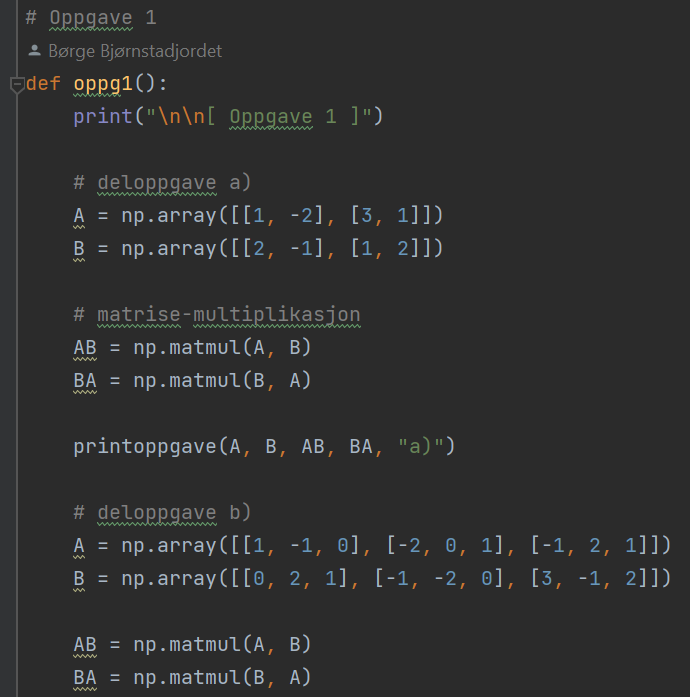
\includegraphics[width=.8\linewidth]{oppg1.png}
  \caption{Oppgave 1 kode}
  \label{fig:sub1}
\end{subfigure}%
\begin{subfigure}{.5\textwidth}
  \centering
  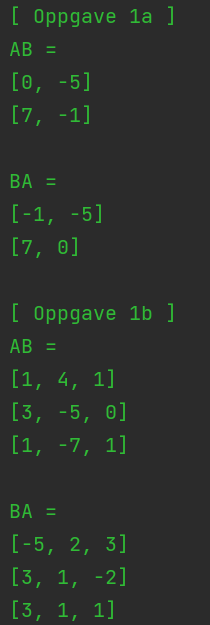
\includegraphics[width=.3\linewidth]{oppg1out.png}
  \caption{Oppgave 1 output}
  \label{fig:sub2}
\end{subfigure}
\caption{Seksjon 1.5 oppgave 1}
\label{fig:test}
\end{figure}

\hfill

\begin{figure}[H]
\centering
\begin{subfigure}{.5\textwidth}
  \centering
  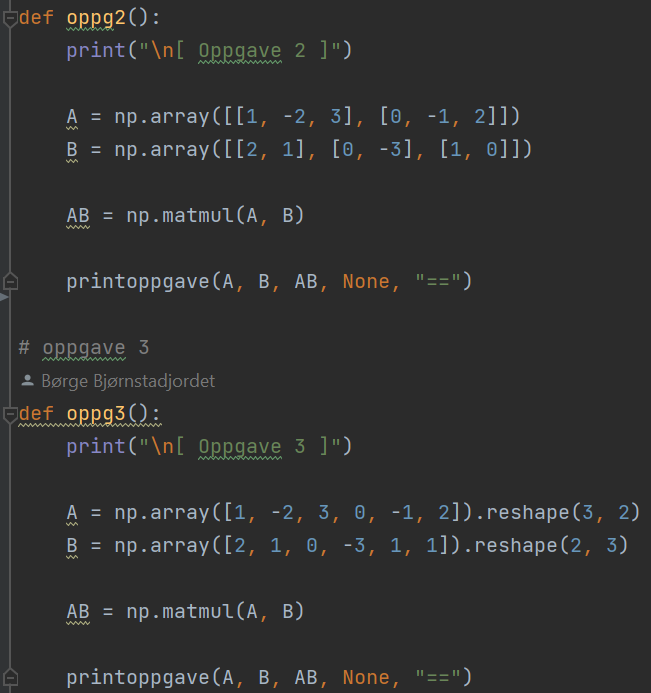
\includegraphics[width=0.8\linewidth]{oppg2-3.png}
  \caption{Oppgave 2 og 3 kode}
  \label{fig:sub1}
\end{subfigure}%
\begin{subfigure}{.5\textwidth}
  \centering
  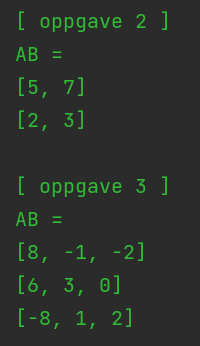
\includegraphics[width=.3\linewidth]{oppg2-3out.png}
  \caption{Oppgave 2 og 3 output}
  \label{fig:sub2}
\end{subfigure}
\caption{Seksjon 1.5 oppgave 2 og 3}
\label{fig:test}
\end{figure}

\newpage

\section*{Seksjon 1.7}

\subsection*{Oppgave 5}

\[ A^{-1} = \begin{pmatrix}
    1 & 4 \\ 2 & 9
\end{pmatrix}\ \quad 
B^{-1} = \begin{pmatrix}
    8 & 3 \\ 2 & 1
\end{pmatrix}\]

Setning 1.7.4 (ii) forteller oss at \( (AB)^{-1} = B^{-1}A^{-1}\), derfor er ...

\[(AB)^{-1} = B^{-1}A^{1} = \begin{pmatrix}
    8 & 3 \\ 2 & 1
\end{pmatrix}\begin{pmatrix}
    1 & 4 \\ 2 & 9
\end{pmatrix} = \begin{pmatrix}
    8 \cdot 1 + 3 \cdot 2 & 8 \cdot 4 + 3 \cdot 9 \\ 2 \cdot 1 + 1 \cdot 2 & 2 \cdot 4 + 1 \cdot 9
\end{pmatrix} = \underline{\begin{pmatrix}
    14 & 59 \\ 4 & 17
\end{pmatrix} = (AB)^{-1}}\]

\hfill

\subsection*{Oppgave 8}

'Dersom A og B er inverterbare, så er den inverse til \((AB)^T\) lik \((A^{-1})^T (B^{-1})^T\)' \\
La A og B være to inverterbare matriser.

Den inverse til \((AB)^T \text{ er lik } (AB)^T)^{-1}\)

Ved setning 1.6.4 (v) har vi at \((AB)^T = B ^T A^T\) \\
- Derfor er \(((AB)^T)^{-1} = (B^T A^T)^{-1}\)

\newline
Ved setning 1.6.4 (v) har vi at \((AB)^T =B^T A^T \) \\
- Derfor er \((AB^T)^{-1}  = (B^TA^T)^{-1}\)

\newline
Ved setning 1.7.6 (ii) har vi at \(AB)^{-1} = B^{-1}A^{-1}\) \\
- Derfor er \((B^T A^T = (B^T)^{-1}(A^T)^{-1}\)

\newline
Ved setning 1.7.6 (iii) har vi at \((A^T)^{-1} = (A^-1)^{-1}\) \\
Derfor er \((A^T)^{-1} \cdot (B^T)^{-1} = (A^{-1})^T \cdot (B^{-1})^T\)

\underline{Derfor er det slik at \((AB)^T\) invers er lik \((A^{-1})^T (B^{-1})^T\)}

\newpage

\section*{Seksjon 1.8}

\subsection*{Oppgave 10}

a)
\[A = \begin{vmatrix}
    3 & -2 & -1 \\ 1 & 4 & 3 \\ 2 & 1 & 7
\end{vmatrix}\]

\[#\#A = 
3 \begin{vmatrix}
    4 & 3 \\ 1 & 7
\end{vmatrix} -
(-2) \begin{vmatrix}
    1 & 3 \\ 2 & 7
\end{vmatrix} +
(-1) \begin{vmatrix}
    1 & 4 \\ 2 & 1
\end{vmatrix}\]
\begin{align*}
    &= 3\cdot(4\cdot7 - 3\cdot1) + 2 \cdot(1\cdot7 - 3\cdot2) - 1\cdot(1\cdot1 - 4\cdot2) \\
    &= 3\cdot(28 - 3) + 2\cdot(7 - 6) -1\cdot(1 - 8) \\
    &= (3\cdot25) + (2\cdot1) + ((-1)\cdot(-7)) \\
    &= 75 + 2 + 7 \\
    &= \underline{84}
\end{align*}

b)
\[B = \begin{vmatrix}
    -2 & 4 & 0 \\ -2 & 3 & 3 \\ 1 & 0 & 4
\end{vmatrix}\]

\[\#B = 
-2\begin{vmatrix}
    3 & 3 \\ 0 & 4
\end{vmatrix} -
4\begin{vmatrix}
    -2 & 3 \\ 1 & 4
\end{vmatrix} + 
0\begin{vmatrix}
    -2 & 3 \\ 1 & 0
\end{vmatrix}\]
\begin{align*}
    &= -2\cdot(3\cdot4 - 3\cdot0) -4\cdot(-2\cdot4 -3\cdot1) + 0 \\
    &= -2\cdot(12 - 0) -4\cdot(-8-3) \\
    &= -2\cdot12 - 4\cdot-11 \\
    &= -24 + 44 \\
    &= \underline{20} \\
\end{align*}

c)
\[C = \begin{vmatrix}
    1 & 2 & 3 \\ -2 & 5 & 4 \\ 3 & -3 & -1
\end{vmatrix}\]

\[\#C = 
1\begin{vmatrix}
    5 & 4 \\ -3 & -1
\end{vmatrix} -
2\begin{vmatrix}
    -2 & 4 \\ 3 & -1
\end{vmatrix} +
3\begin{vmatrix}
    -2 & 5 \\ 3 & -3
\end{vmatrix}\]
\begin{align*}
    &= 1 \cdot ( (5\cdot-1) - (4\cdot-3) ) -2 \cdot ( (-2\cdot-1) - (4\cdot3) ) +3 \cdot ( (-2\cdot-3) - (5\cdot3) ) \\
   &=  1 \cdot (-5 - (-12)) -2 \cdot (2 - 12) +3  \cdot (6 - 15) \\
   &= (1 \cdot 7) + (-2 \cdot -10) + (3 \cdot -9) \\
   &= 7 + 20 - 27 \\
   &= \underline{0}
\end{align*}


\end{document}
